\section{Experimental Results\label{sec:radar.results}}

\FloatBarrier


\thecontrib serves multiple objectives at once:
\begin{enumerate*}[(a)]
    \item maintaining high performance on \emph{practical} \gls{niid} data,
    \item correctly identifying and weighting low-quality contributions, and
    \item mitigating the impact of label-flipping attacks.
\end{enumerate*}
As a result, we select relevant baselines from the literature to evaluate each of \thecontrib's abilities.
We use \texttt{FedAvg}~\cite{mcmahan_Communicationefficientlearningdeep_2017} (abbreviated \texttt{FA}) to highlight the existing issues with statistical heterogeneity, using the setup provided by Flower~\cite{flower_fedavg_impl}.
Because \thecontrib can be partially assimilated as a clustered \texttt{FedAvg} variant, we also consider a theoretical setup where participants are clustered based on their original data distribution, and one instance of \texttt{FedAvg} is executed per cluster.
We refer to it as \emph{Clustered} $\texttt{FedAvg}$ or \texttt{FC}.
To highlight \thecontrib's ability to compare with Sybil-focused mitigation strategies, we compare it with \texttt{FoolsGold}~\cite{fung_LimitationsFederatedLearning_2020} (also designated \texttt{FG}).
We reuse the authors' code~\cite{foolsgold_dl_impl}, and adapt it to model updates, since \texttt{FoolsGold} was originally implemented on \texttt{FedSGD}.
The following sections cover these topics using the scenarios laid out in \Cref{sec:radar.methodo.scenarios}.
Like the others, \thecontrib is abbreviated as \texttt{RA} when needed.


\subsection{Heterogeneity\label{sec:radar.results.heterogeneity}}


\begin{table}
  \centering
  \caption{
    \emph{Rand index between \thecontrib's clustering and two partitions of reference, under various scenarios.} 
    Partition \textbf{(A)} contains only benign participants grouped according to their respective dataset. 
    Partition \textbf{(B)} contains attackers placed in a separated group in addition to benign participants. 
    \label{tbl:radar.rand_clustering}
  }

  \setlength\tabcolsep{0.8ex}
  \begin{tabular}{lrcccc}
    \toprule
    \multicolumn{3}{c}{\textbf{Scenario}} && \multirow{2}{*}{\textbf{Partition (A)}} & \multirow{2}{*}{\textbf{Partition (B)}} \\
    \textit{Category} & \textit{Noisiness} & \textit{Target} && & \\
    \midrule % ---------------------------------
    \texttt{Benign} & & && 1.00 & 1.00 \\ 
    
    \midrule[.1pt] % ---------------------------------
    \texttt{Lone } & $\le$100 & T && 1.00 & 0.97 \\
    \texttt{Lone} & $\le$95 & U && 1.00 & 0.97 \\
    \texttt{Lone} & 100 & U  && 1.00 & 1.00 \\  
    
    \midrule[.1pt] % ---------------------------------
    \texttt{Collud. min.} & $\le$100 & T && 1.00 & 0.97 \\
    \texttt{Collud. min.} & $\le$90 & U && 1.00 & 0.97 \\
    \texttt{Collud. min.} & 100 & U && 1.00 & 1.00 \\

    \midrule[.005em] % ---------------------------------
    \texttt{Collud. maj.} & $\le$100 & T && 1.00 & 0.96 \\
    \texttt{Collud. maj.} & $\le$90 & U && 1.00 & 0.96 \\
    \texttt{Collud. maj.} & 100 & U && 1.00  & 1.00 \\
    \bottomrule % ---------------------------------
  \end{tabular}
\end{table}

\begin{table}
  \centering
  \caption{
      \emph{Effect of different attack configurations (\texttt{100T/U}) on all baselines.}
      The \acrfull{asr} is computed over the targeted classes in targeted attacks, and over all samples otherwise (see \Cref{sec:radar.methodo.metrics}).
      \texttt{RA} is \thecontrib, \texttt{FG} is \texttt{FoolsGold}, $\texttt{FA}$ is \texttt{FedAvg} (on \emph{all} participants), and \texttt{FC} is \texttt{FedAvg} ideally clustered per dataset.
      The \gls{asr} of benign runs is provided as a baseline.
      \thecontrib's limiting scenario is marked $\ddagger$.
      \label{tbl:radar.baselines_results}
  }

  \newcolumntype{T}{>{\footnotesize}r}

  \setlength\tabcolsep{1ex}
  \begin{tabularx}{\textwidth}{lX|TTTT|TTTT}
    \toprule % ---------------------------------
    \multicolumn{2}{c|}{\multirow{2}{*}{\textbf{Scenario}}} & \multicolumn{4}{c|}{\textbf{Mean accuracy} (\%)} & \multicolumn{4}{c}{\textbf{\gls{asr}} (\%)} \\
    & & \multicolumn{1}{c}{\texttt{RA}} & \multicolumn{1}{c}{\texttt{FG}} & \multicolumn{1}{c}{\texttt{FA}} & \multicolumn{1}{c|}{\texttt{FC}} & \multicolumn{1}{c}{\texttt{RA}} & \multicolumn{1}{c}{\texttt{FG}} & \multicolumn{1}{c}{\texttt{FA}} & \multicolumn{1}{c}{\texttt{FC}} \\
    \midrule % ---------------------------------
    % TARGETED ATTACKS
    \multicolumn{2}{l|}{\textbf{Targeted} (\texttt{100T})} & & & & & & & & \\
                & \texttt{Benign}       & 99.07 & 55.04 & 79.49 & \textbf{99.24} & \textbf{0.00} &  5.17 & 5.10 &  0.09 \\
                & \texttt{Lone}         & 99.06 & 60.51 & 77.38 & \textbf{99.22} & \textbf{0.00} & 93.82 & 6.73 &  0.45 \\
                & \texttt{Collud. min.} & \textbf{98.96} & 54.64 & 78.48 & 98.33 & \textbf{0.00} &  2.97 & 9.99 & 53.40 \\
    $\ddagger$  & \texttt{Collud. maj.} & \textbf{98.28} & 85.10 & 79.40 & 98.22 & 73.39 & \textbf{8.10} & 17.65 & 59.36 \\
    \midrule % ---------------------------------
    % UNTARGETED ATTACKS
    \multicolumn{2}{l|}{\textbf{Untargeted} (\texttt{100U})} & & & & & & & & \\
    & \texttt{Benign}        & 99.07 & 55.04 & 79.49 & \textbf{99.24} & 0.09  & 0.39 & 33.30 & \textbf{0.06} \\
    & \texttt{Lone}          & 98.96 & 49.56 & 78.38 & \textbf{99.22} &\textbf{0.08} & 99.89 & 54.70 & 0.12 \\
    & \texttt{Collud. min.}  & \textbf{98.98} & 49.67 & 72.47 & 97.69 & 0.10 & \textbf{0.04} & 44.53 & 6.26 \\
    & \texttt{Collud. maj.}  & \textbf{98.96} & 69.09 & 81.87 & 75.66 & \textbf{0.08} & 38.98 & 59.49 & 94.36 \\          
    \bottomrule % ---------------------------------
  \end{tabularx}
\end{table}


Because our use case implies that some participants share similar data distributions, we expect \thecontrib's clustering component to limit the impact of heterogeneity by grouping similar participants together.
To evaluate our approach, we compare the partition created by \thecontrib's clustering algorithm with one where participants are grouped according to their dataset of origin.
This partition is presented as Partition A in \Cref{tbl:radar.rand_clustering}.
The constant Rand index of 1.0 indicates that all participants are correctly grouped, regardless of the considered evaluation scenario.
This validates the idea that similarity between evaluations can be used to regroup participants. 

In addition to managing heterogeneity, it is critical that the countermeasures deployed in \thecontrib do not negatively impact performance.
Specifically, the reputation system must not unfairly penalize legitimate participants because of their potential differences.
\Cref{fig:reput_byzantine.benign} presents the weights provided by the reputation system for the aggregation. 
In the \texttt{Benign} scenario, the 5 participants originating from the Bot-IoT dataset do have equal weights, confirming that none of them is penalized by the reputation system.
Furthermore, \Cref{tbl:radar.baselines_results} indicates that \thecontrib's mean accuracy is superior to \texttt{FoolsGold}'s and $\texttt{FedAvg}$, as both baselines falter in practical \gls{niid} use cases.
\thecontrib almost matches the results of \texttt{FC}, which is ideally clustered by design.
Overall, \texttt{FoolsGold}, a reference Byzantine-resilient \gls{fl} strategy tailored for \gls{niid} settings, falters in \emph{practical} \gls{niid} settings, where \thecontrib strives.


\subsection{Handling data quality\label{sec:radar.results.quality}}

Another goal for \thecontrib is to handle contributions of various quality.
This objective is mostly represented by scenarios of \Cref{cat:lone} (\texttt{Lone}), as we consider that coordinated faults are improbable for legitimate participants.
In this configuration, we expect the Byzantine participant to be either, put in a cluster of its own, or penalized by the reputation system.
To verify the former, we compare the partition made by \thecontrib with another where Byzantines are segregated in an additional cluster (see Partition B in \Cref{tbl:radar.rand_clustering}).
Here, a Rand index lower than 1.0 implies that Byzantine participants have been grouped with legitimate ones of the same dataset, which is the case in most scenarios of the \texttt{Lone} category.
However, the noisiest untargeted faults (\texttt{Lone~$>$95U}) result in the Byzantine participant being placed in his own separate cluster, thus neutralizing its impact on the other participants.
Note that the hyperparameters of the clustering algorithm could be tuned so that attackers with lower \emph{noisiness} would be separated, notably the threshold factor $\beta$ and the cross-evaluation metric (see \Cref{tbl:radar.hyperparameters}).

When Byzantine participants are grouped with benign ones, we rely on the reputation system to identify and diminish the impact of their contributions.
The weights given by the reputation system can be seen in \Cref{fig:reput_byzantine.lone}, where the Byzantine client is heavily penalized in the \texttt{Lone~100T} scenario.
The effect of the clustering and reputation system are also apparent in \Cref{tbl:radar.baselines_results}, where the \gls{asr} for both \texttt{Lone~100T} and \texttt{Lone~100U} are comparable to the benign case, underlining \thecontrib resilience.
The results in \Cref{fig:asr_multiple_baselines} confirm this trend: \thecontrib maintains a low \gls{asr} in most configurations.
As a result, \thecontrib demonstrates its ability to mitigate isolated Byzantine faults, regardless of their intensity. 

The same cannot be said for \texttt{FoolsGold}'s, which aims at providing a single global model.
Further, by construction, it identifies groups of similar participants as colluding attackers and considers that only the faulty participant is legitimate. 
This appreciation error leads \texttt{FoolsGold} to have the worst attack success rate among all tested baselines, even when compared against the naive \texttt{FedAvg} approach.


\begin{figure*} % Reputation weights as function of the number of byzantines
  \centering
  \begin{subfigure}[t]{0.4\linewidth}
    \centering
    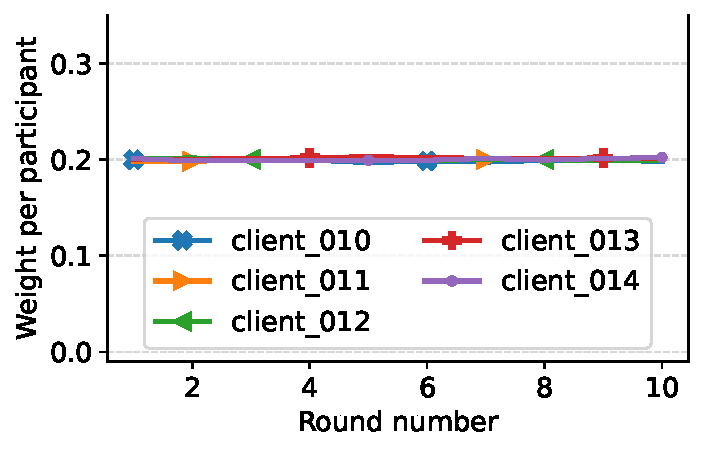
\includegraphics[trim=0 0 10pt 0,clip,width=\linewidth]{figures/reput/benign_expanded.pdf}
    \caption{\footnotesize\texttt{Benign}.}
    \label{fig:reput_byzantine.benign}
  \end{subfigure}
  \qquad 
  \begin{subfigure}[t]{0.4\linewidth}
    \centering
    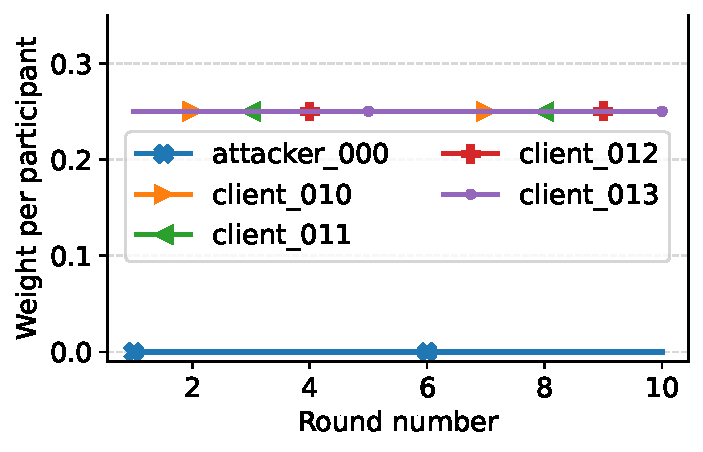
\includegraphics[trim=0 0 10pt 0,clip,width=\linewidth]{figures/reput/lone_loud_expanded.pdf}
    \caption{\footnotesize\texttt{Lone~100T}.}
    \label{fig:reput_byzantine.lone}
  \end{subfigure}

  \begin{subfigure}[t]{0.4\linewidth}
    \centering
    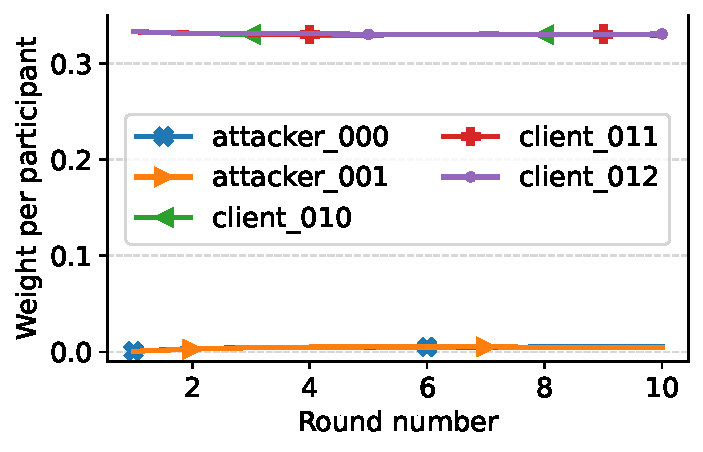
\includegraphics[trim=0 0 10pt 0,clip,width=\linewidth]{figures/reput/byzantine_minority_loud_expanded.pdf}
    \caption{\footnotesize\texttt{Colluding~minority~100T}.}
    \label{fig:reput_byzantine.minority}
    \end{subfigure}
  \qquad 
  \begin{subfigure}[t]{0.4\linewidth}
    \centering
    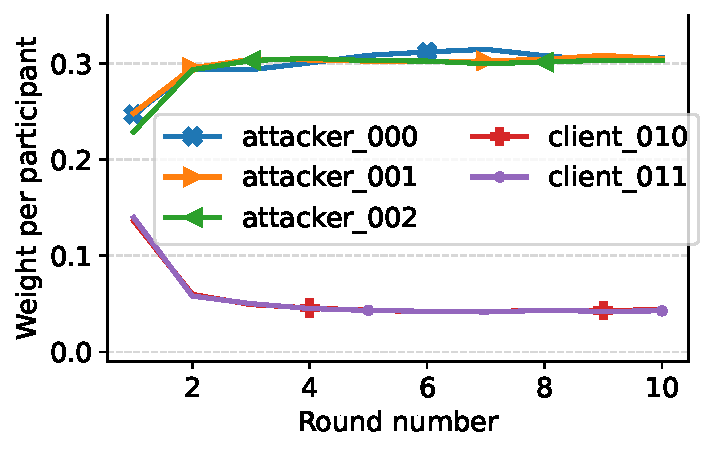
\includegraphics[trim=0 0 10pt 0,clip,width=\linewidth]{figures/reput/byzantine_majority_loud_expanded.pdf}
    \caption{\footnotesize\texttt{Colluding~majority~100T}.}
    \label{fig:reput_byzantine.majority}
  \end{subfigure}
  \caption{
    \emph{Aggregation weights $\weight$ for the participants coming from the BoT-IoT dataset depending on the number of Byzantines (\texttt{100T}). } 
    Byzantines are correctly penalized when they are a minority, but gain precedence when they become the majority.
  }
  \label{fig:reput_byzantine}
\end{figure*}

\begin{figure*} % Increasing percent of poisoning
  \centering 
  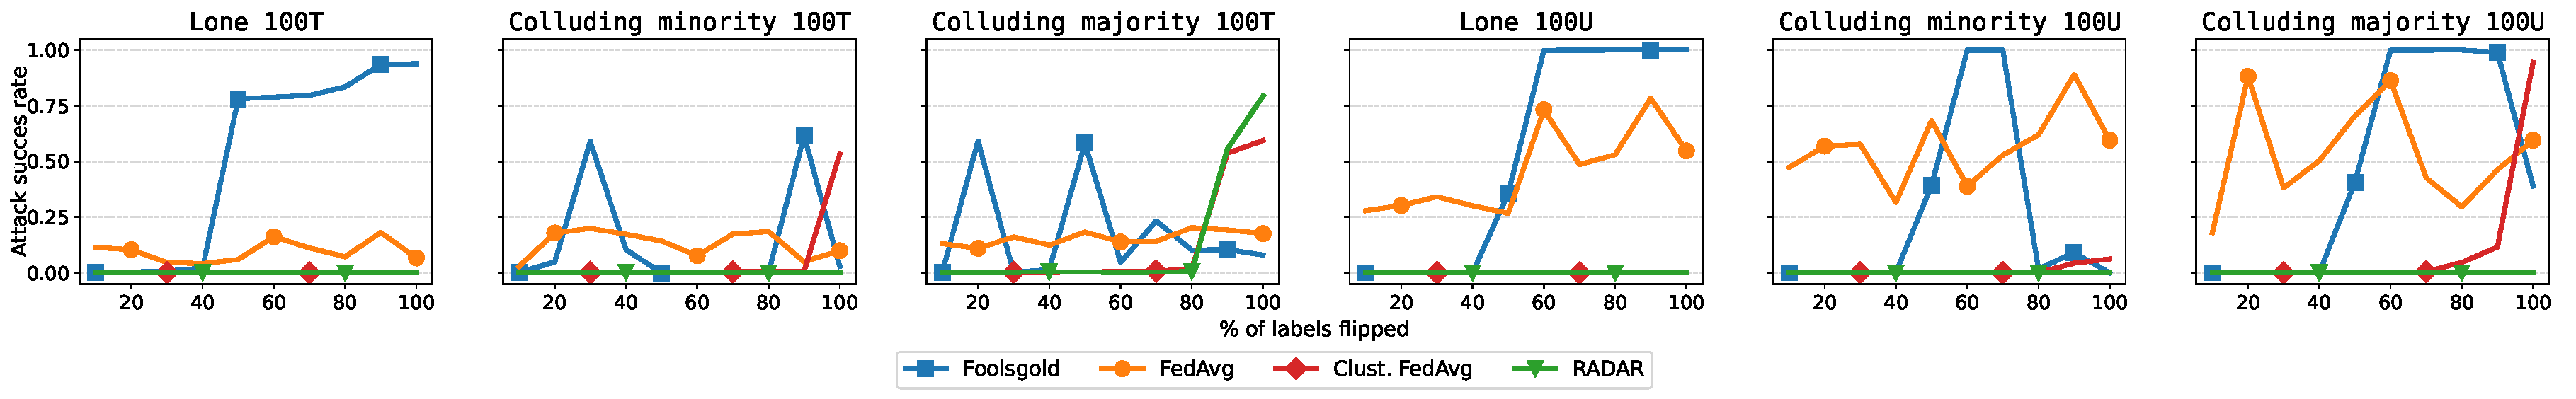
\includegraphics[width=\linewidth]{figures/poisoning/asr_multiple_baselines.pdf}    
  \caption{
    \emph{\Acrfull{asr} of the different baselines.}
    Even though attackers are a majority, they gain weight precedence only for higher poisoning rates ($>$90\%).  
  }
  \label{fig:asr_multiple_baselines}
\end{figure*}

\begin{figure*} % ASR of the different attacks 
  \centering     
    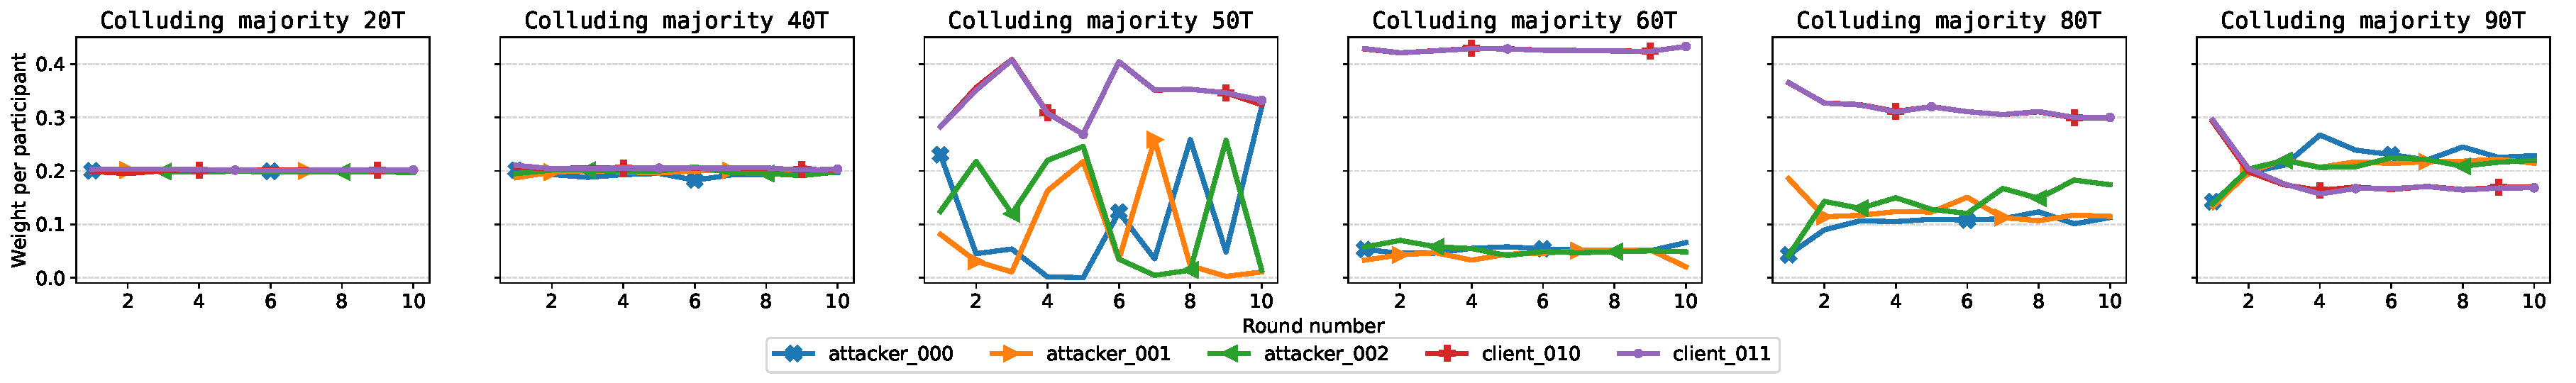
\includegraphics[width=\linewidth]{figures/reput/majority_attackers_targeted_multiple_percents.pdf}    
  \caption{
    \emph{Aggregation weights $\weight$ per participant of the poisoned cluster (\texttt{Colluding majority T}).}
    Even though attackers are a majority, they gain weight precedence only for higher poisoning rates ($\ge$90\%).  
  }
  \label{fig:majority_targeted_flipping_effect}
\end{figure*}


\subsection{Label flipping attacks\label{sec:radar.results.flipping}}

We evaluate the resistance to label-flipping attacks using two different scenarios.
First, we consider that \texttt{Colluding Byzantines} can only refer to attackers, as it is unlikely that the very same fault happens over multiple clients at the same time.
Second, the \texttt{Lone~100U} scenario, as it is similarly unlikely that for an \emph{honest-but-neglectful} participant to misclassify the entirety of its data.

Like discussed in \Cref{sec:radar.results.quality}, the clustering algorithm separates the noisiest attacks from the rest.
This is true regardless of the number of attackers, as confirmed by the results in \Cref{tbl:radar.rand_clustering}.
For untargeted faults with at least 95\% \emph{noisiness}, the Rand index at round 10 stays equal to 1.0.
This means that for those loud attacks, attackers are separated from benign participants, hence negating their poisoning effect.
This is a critical result for \thecontrib, as this mitigation occurs for \emph{any number of attackers}, even if they outnumber benign participants.
However, the attackers in \texttt{Colluding T} scenarios are placed with legitimate participants in the same cluster. 


\paragraph*{Minority of attackers\label{sec:radar.results.flipping.minority}}

The \texttt{Colluding minority} class (\Cref{cat:colluding}) contains scenarios where 2 out of 5 participants instantiated in Bot-IoT perpetrate label-flipping attacks.
Here, the results depicted in \Cref{fig:reput_byzantine.minority} indicate that the attackers are heavily penalized by the reputation system. 
This is coherent with the results in \Cref{tbl:radar.baselines_results} for these scenarios, where we can see that \thecontrib indeed fend off attackers with an \gls{asr} of 0.0.
Among the other baselines, \texttt{FedAvg} is especially affected, since it does not have any protection against such attacks.
This is also true for our theoretical baseline \texttt{FC}, although the effect is logically limited to participants using the Bot-IoT dataset.
\texttt{FoolsGold}, on the other hand, detects the attackers since they are similar and thus manages to discard the attack, obtaining a rather low \gls{asr} of 2.97\%.
Unfortunately, it also detects benign members from the other clusters as colluding attackers and thus train on BoT-IoT only, leading to a very low 54.64\% accuracy overall.


\paragraph*{Majority of attackers\label{sec:radar.results.flipping.majority}}

The \texttt{Colluding majority 100T} scenario, with 3 attackers out of 5 participants, sees the attackers gain precedence.
\Cref{fig:reput_byzantine.majority} clearly illustrates this phenomenon, where the legitimate participants' weights drop as the reputation system favors the attackers.
This is a known limit of the reputation system, which favors the majority by construction.
This is further illustrated in~\Cref{fig:trustfids_accuracy_missrate_distribution}: a steeper drop in accuracy and miss rate occurs when attackers outnumber benign participants in one cluster.
However, the metric distribution over the participants highlights that the other clusters remain unaffected, and that the majority of benign participants continues to perform well.
Furthermore, as illustrated in \Cref{fig:asr_multiple_baselines,fig:majority_targeted_flipping_effect}, the \emph{noisiness} of attackers must exceed 80\% for attackers to poison the cluster's model.
Consequently, while this scenario highlights a limitation of \thecontrib, it is significantly constrained.


\paragraph*{Impact of the attack timing\label{sec:radar.results.flipping.timing}}

Additionally, \Cref{fig:redemption_decrease} depicts how the reputation system reacts to participants that change their \emph{noisiness} over time. 
\Cref{fig:redemption_byzantine_min} features a \texttt{Colluding minority 100T} scenario where the noisiness drops to 0\% at round 3. 
The system forgives attackers approximately four rounds after they adapted their behavior.
This rather short delay depends on the chosen $\lambda$ history parameter of our reputation system (see \Cref{tbl:radar.hyperparameters}). 
On the contrary, \Cref{fig:increment_byzantine_min} showcases \texttt{Colluding minority T} attackers going from 0 to 100\% noisiness over the course of a few rounds.
The reputation system detects and penalizes them at round 5 when the noisiness reaches 60\%. 
This in phase with the conclusions of \Cref{fig:asr_multiple_baselines,fig:majority_targeted_flipping_effect}: for lower noisiness levels, the attackers have no effect. 
The reputation system thus detects attackers only when they start to present a threat to the global model's performance. 


\subsection{Synthesis\label{sec:radar.results.synthesis}}

First, the results highlight the relevance of clustering in \emph{practical \gls{niid}} use cases, as attacks are confined to the cluster attackers have been assigned to.
This is particularly visible in the performance of \thecontrib and the clustered \texttt{FedAvg} variant, which both maintain high accuracy overall by providing each community with a specific model.
This is true even in the presence of Byzantine faults or attackers.
However, since $\texttt{FC}$ does not implement any mitigation strategy, its performance quickly degrades with the quality of the contributions, especially in the presence of colluding attackers (as illustrated by \Cref{fig:asr_multiple_baselines}).

The results in \Cref{tbl:radar.baselines_results} also emphasize on \texttt{FoolsGold}'s unsuitability for \emph{practical \gls{niid}} use cases, where groups of participants sharing similar distributions can exist.
Especially in a \texttt{Lone} scenario, any groups of similar participants are considered as colluding attackers and penalized, leading to high \gls{asr}, as only the attacker is considered as legitimate.
Similarly, in \texttt{Colluding majority T/U} scenarios, \texttt{FoolsGold} penalizes all the other clusters, leading to a model trained on Bot-IoT only.
Overall, \thecontrib presents the most consistent results, with high accuracy and low \gls{asr} in most scenarios, only failing against a majority of extremely \emph{noisy} colluding attackers that still managed to get similar enough to be grouped with benign participants.

\begin{figure}
  %\centering 
  \begin{subfigure}[t]{1.0\linewidth}
    \centering 
    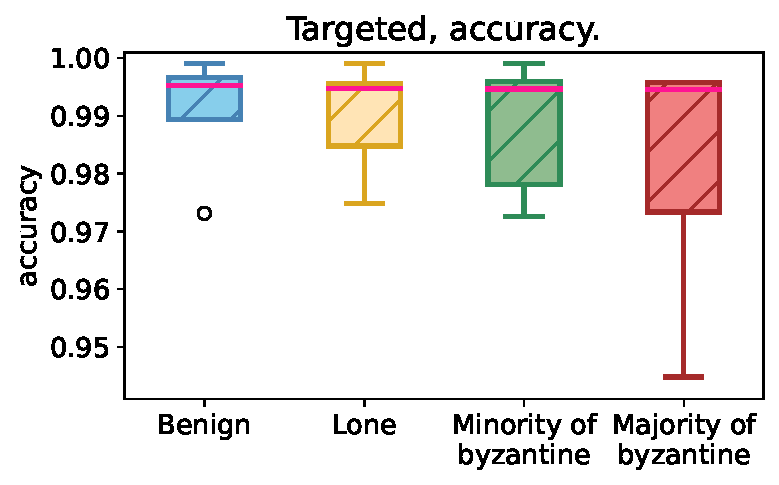
\includegraphics[width=0.4\linewidth]{figures/poisoning/trusfids_targeted_acc_all_distibutions.pdf} 
    \qquad   
    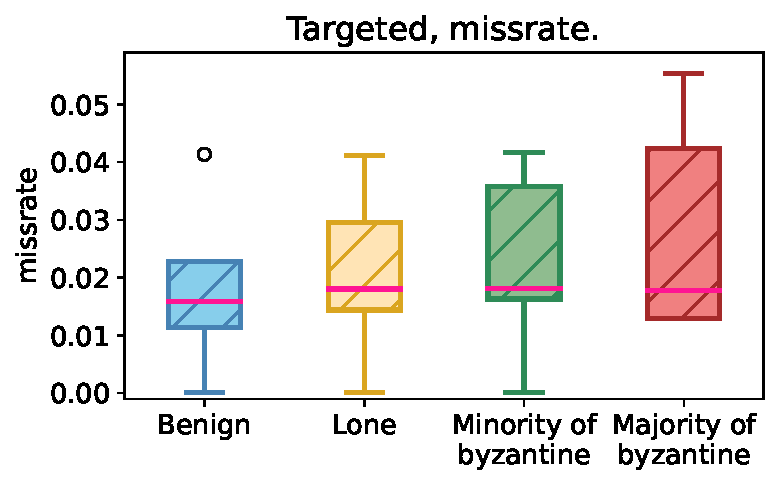
\includegraphics[width=0.4\linewidth]{figures/poisoning/trusfids_targeted_missrate_all_distibutions.pdf}   
\end{subfigure}
  \caption{
    \emph{\thecontrib's metric distribution among participants in different scenarios (\texttt{100T}).}
    The accuracy's and miss rate's lower bounds suddenly drop when attackers outnumber benign participants in the affected cluster.
    Indeed, clients in other clusters are unaffected by the poisoning.
  }
  \label{fig:trustfids_accuracy_missrate_distribution}
  
\end{figure}


\begin{figure} % Reputation system redemption and late
  \centering 
  \begin{subfigure}[t]{.4\linewidth}
    \centering 
    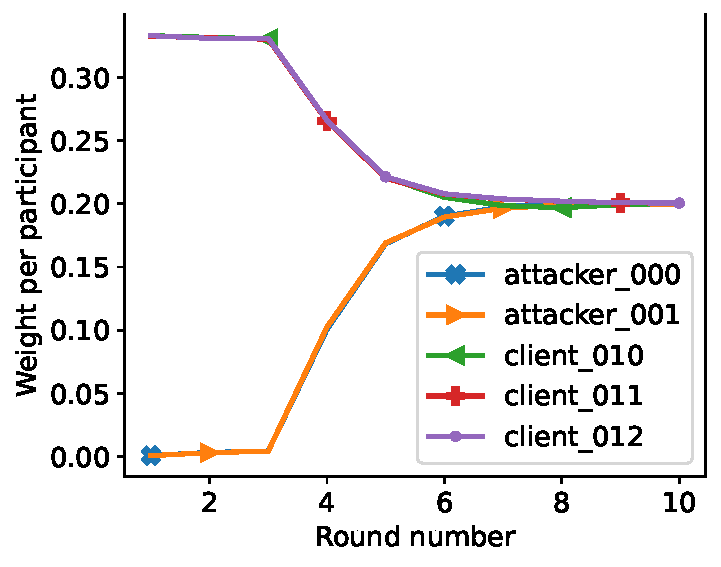
\includegraphics[trim=0 0 10pt 0,clip,width=\linewidth]{figures/reput/redemption_byzantine_min.pdf}    
    \caption{\footnotesize
      Attackers act with 100\% \emph{noisiness}, but become benign on round 3.
    }
    \label{fig:redemption_byzantine_min}
  \end{subfigure}
  \qquad
  \begin{subfigure}[t]{.4\linewidth}
    \centering 
    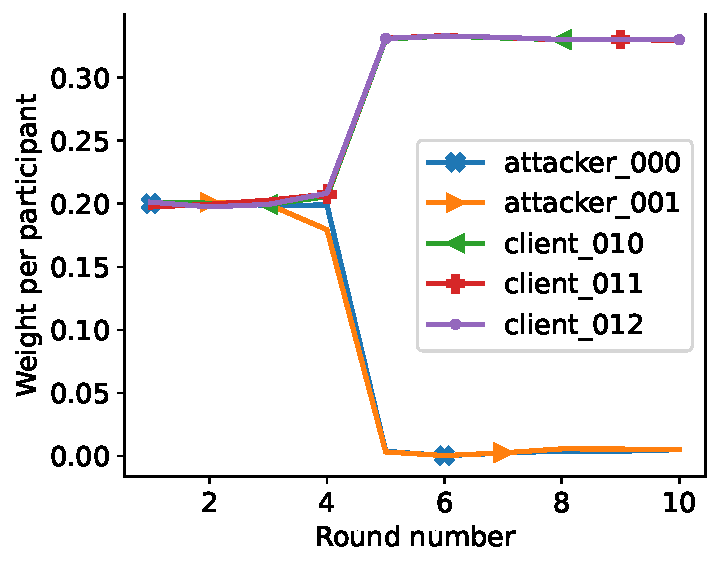
\includegraphics[trim=0 0 10pt 0,clip,width=\linewidth]{figures/reput/increment_byzantine_min.pdf}
    \caption{\footnotesize
      Attackers start benign, and increase \emph{noisiness} by 20\% each round when $r\geq3$.
    }
    \label{fig:increment_byzantine_min}
  \end{subfigure}
  \caption{
    \emph{Aggregation weights $\weight$ per participant of the poisoned cluster (\texttt{Colluding minority T}).}
    Attackers are forgiven over time, and the reputation system reacts quickly to newly detected attackers.
  }
  \label{fig:redemption_decrease}

\end{figure}







